\documentclass[UTF8]{ctexart}

\usepackage{listings}
\usepackage{color}
\usepackage{amsmath} 
\usepackage{graphicx}
\usepackage[colorlinks,linkcolor=blue]{hyperref}

\definecolor{dkgreen}{rgb}{0,0.6,0}
\definecolor{gray}{rgb}{0.5,0.5,0.5}
\definecolor{mauve}{rgb}{0.58,0,0.82}

\lstset{ %
    aboveskip=3mm,
    belowskip=3mm,
    showstringspaces=false,
    columns=flexible,
    basicstyle={\small\ttfamily},
    numbers=left,
    numberstyle=\tiny\color{gray},
    keywordstyle=\color{blue},
    commentstyle=\color{dkgreen},
    stringstyle=\color{mauve},
    breaklines=true,
    breakatwhitespace=true,
    tabsize=3
}

\title{笔记 22-10-20}
\author{李肖}
\date{2022 年 10 月 20 日}

\begin{document}

% File cover
\maketitle

\section{图算法}

\subsection{图的表示}
\[Graph: G(E, V)\]
其中:E 是 边的集合,V 是点的集合,比如说

\[V: \{A, B, C\}\]
\[E: \{(A, B), (A, C), (B, C), (B, A), (C, A), (C, B)\}\]

\subsection{图的种类}
\begin{itemize}
    \item directed graph 有向图
    \item undirected graph 无向图
\end{itemize}

\subsection{图在计算机中的存储}

\noindent
\textbf{临接矩阵}

\[
    G = \begin{bmatrix}
        0 & 1 & 1 \\
        0 & 0 & 0 \\
        0 & 1 & 0
    \end{bmatrix}
\]

\vskip 0.4cm
\noindent
其中 1 代表连通,0 代表不连通

\vskip 1cm
\noindent
\textbf{临接表}
\vskip 0.5cm
\begin{figure}[htbp]
    \centering
    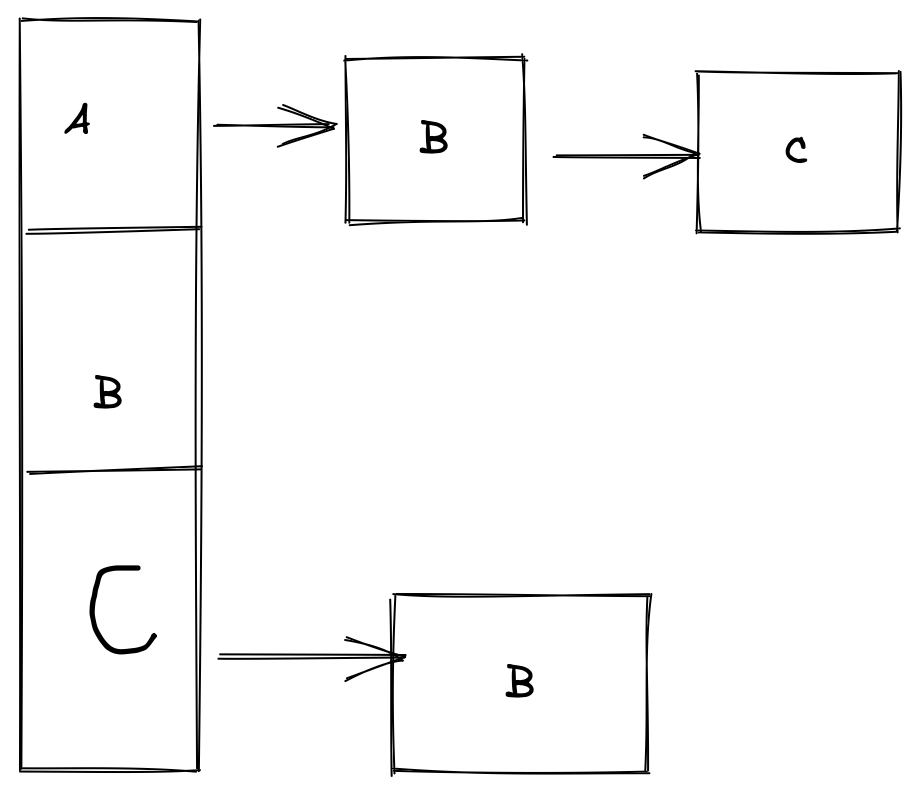
\includegraphics[scale=0.2]{./img/list.png}
\end{figure}


\noindent
\textbf{两种表的优缺点:}
\begin{itemize}
    \item 临接矩阵查找连通快,但是存储空间大
    \item 临接表查找连通慢,但是存储空间小
\end{itemize}

\subsection{问题应用}

\subsubsection{八皇后问题}

\noindent
使用 DFS 来解决问题。

\vskip 0.2cm
\noindent
\textbf{空间优化:}

因为列不能重复,所以说只要用一个数组就能存图

\[Arr = [2, 4, 1, 3]\]

在上面的这个数组中,第一行的皇后在第二列,
第二行的皇后在第 4 列,第三行的皇后在第一列……


\end{document}